\documentclass{scrreprt}

\usepackage{aligned-overset}
\usepackage{amsmath}
\usepackage{amsthm}
\usepackage{amssymb}
\usepackage{bm}
\usepackage[shortlabels]{enumitem}
\usepackage{hyperref}
\usepackage[utf8]{inputenc}
\usepackage{multicol}
\usepackage{mathtools}
\usepackage{pdflscape}
\usepackage{pifont}
\usepackage{physics}
\usepackage{polynom}
\usepackage{tabularx}
\usepackage[table]{xcolor}
\usepackage{titling}
\usepackage{fancyhdr}
\usepackage{xfrac}
\usepackage{pgfplots}

\pgfplotsset{compat = newest}
\usetikzlibrary{arrows, arrows.meta}
\usetikzlibrary{calc}

\author{Karsten Lehmann \\ 4935758}
\date{WiSe 2024/25}
\title{Nachbereitungsaufgaben 13\\INF-B-110, Diskrete Strukturen}

\setlength{\headheight}{26pt}
\pagestyle{fancy}
\fancyhf{}
\lhead{\thetitle}
\rhead{\theauthor}
\lfoot{\thedate}
\rfoot{Seite \thepage}


\begin{document}
\paragraph{N13}
\begin{enumerate}[(a)]
\item Ein Baum $G = \qty\big(V, E)$ mit Knotenmenge
  $V = \qty\big{0, 1, \ldots, 8}$ ist durch den Prüfercode
  $\qty\big(2, 8, 1, 0, 0, 4, 2)$ gegeben.
  \begin{enumerate}[(1)]
  \item Bestimmen Sie aus dem Prüfercode, welche Knoten Blätter des Baumes sind.

    \subparagraph{Lsg.} Nach Lemma 107 der Vorlesung, \emph{``Sei
      $\qty\big(V, E)$ ein Baum.
      Die Blätter von $\qty\big(V, E)$ sind genau diejenigen Knoten, die im
      Prüfercode nicht vorkommen.''} hat der Baum die Blätter
    $\qty\big{3, 5, 6, 7}$.

  \item Zeichnen Sie ein Diagramm des Baumes $G$.

    \subparagraph{Lsg.} \phantom{\null}

    \begin{tikzpicture}
      \node[circle, draw, inner sep=0pt, minimum size=1mm, label=left:{$5$}] (5) at (0,0) {};
      \node[circle, draw, inner sep=0pt, minimum size=1mm, label=above:{$8$}] (8) at (1,0) {};
      \node[circle, draw, inner sep=0pt, minimum size=1mm, label=below:{$2$}] (2) at (2,0) {};
      \node[circle, draw, inner sep=0pt, minimum size=1mm, label=above:{$3$}] (3) at (2,1) {};
      \node[circle, draw, inner sep=0pt, minimum size=1mm, label=above:{$4$}] (4) at (3,0) {};
      \node[circle, draw, inner sep=0pt, minimum size=1mm, label=below:{$0$}] (0) at (4,0) {};
      \node[circle, draw, inner sep=0pt, minimum size=1mm, label=above:{$7$}] (7) at (4,1) {};
      \node[circle, draw, inner sep=0pt, minimum size=1mm, label=above:{$1$}] (1) at (5,0) {};
      \node[circle, draw, inner sep=0pt, minimum size=1mm, label=right:{$6$}] (6) at (6,0) {};

      \draw (5) -- (8) -- (2) -- (4) -- (0) -- (1) -- (6);
      \draw (3) -- (2);
      \draw (7) -- (0);
    \end{tikzpicture}

  \item Wie ändert sich der Prüfercode, wenn der Baum durch den Knoten 9 und die
    Kante $\qty\big{0, 9}$ erweitert wird?

    \subparagraph{Lsg.} \phantom{\null}

    \begin{minipage}{.3\textwidth}
      \begin{tikzpicture}[scale=0.5]
        \node[circle, inner sep=0pt, minimum size=5mm, fill, blue!20] at (2, 1) {};
        \node[circle, inner sep=0pt, minimum size=5mm, fill, red!20] at (2, 0) {};

        \node[circle, draw, inner sep=0pt, minimum size=1mm, label=left:{$5$}] (5) at (0,0) {};
        \node[circle, draw, inner sep=0pt, minimum size=1mm, label=above:{$8$}] (8) at (1,0) {};
        \node[circle, draw, inner sep=0pt, minimum size=1mm, label=below:{$2$}] (2) at (2,0) {};
        \node[circle, draw, inner sep=0pt, minimum size=1mm, label=above:{$3$}] (3) at (2,1) {};
        \node[circle, draw, inner sep=0pt, minimum size=1mm, label=above:{$4$}] (4) at (3,0) {};
        \node[circle, draw, inner sep=0pt, minimum size=1mm, label=below:{$0$}] (0) at (4,0) {};
        \node[circle, draw, inner sep=0pt, minimum size=1mm, label=above:{$7$}] (7) at (4,1) {};
        \node[circle, draw, inner sep=0pt, minimum size=1mm, label=above:{$1$}] (1) at (5,0) {};
        \node[circle, draw, inner sep=0pt, minimum size=1mm, label=right:{$6$}] (6) at (6,0) {};
        \node[circle, draw, inner sep=0pt, minimum size=1mm, label=right:{$9$}] (9) at (5,-1) {};

        \draw (5) -- (8) -- (2) -- (4) -- (0) -- (1) -- (6);
        \draw (3) -- (2);
        \draw (7) -- (0) -- (9);

        \node at (2, -2.5) {\colorbox{red!20}{$\qty\big(2)$}};
      \end{tikzpicture}
    \end{minipage}
    \begin{minipage}{.3\textwidth}
      \begin{tikzpicture}[scale=0.5]
        \node[circle, inner sep=0pt, minimum size=5mm, fill, blue!20] at (0, 0) {};
        \node[circle, inner sep=0pt, minimum size=5mm, fill, red!20] at (1, 0) {};

        \node[circle, draw, inner sep=0pt, minimum size=1mm, label=left:{$5$}] (5) at (0,0) {};
        \node[circle, draw, inner sep=0pt, minimum size=1mm, label=above:{$8$}] (8) at (1,0) {};
        \node[circle, draw, inner sep=0pt, minimum size=1mm, label=below:{$2$}] (2) at (2,0) {};
        \node[circle, draw, inner sep=0pt, minimum size=1mm, label=above:{$4$}] (4) at (3,0) {};
        \node[circle, draw, inner sep=0pt, minimum size=1mm, label=below:{$0$}] (0) at (4,0) {};
        \node[circle, draw, inner sep=0pt, minimum size=1mm, label=above:{$7$}] (7) at (4,1) {};
        \node[circle, draw, inner sep=0pt, minimum size=1mm, label=above:{$1$}] (1) at (5,0) {};
        \node[circle, draw, inner sep=0pt, minimum size=1mm, label=right:{$6$}] (6) at (6,0) {};
        \node[circle, draw, inner sep=0pt, minimum size=1mm, label=right:{$9$}] (9) at (5,-1) {};

        \draw (5) -- (8) -- (2) -- (4) -- (0) -- (1) -- (6);
        \draw (7) -- (0) -- (9);

        \node at (2, -2.5) {\colorbox{red!20}{$\qty\big(2, 8)$}};
      \end{tikzpicture}
    \end{minipage}
    \begin{minipage}{.3\textwidth}
      \begin{tikzpicture}[scale=0.5]
        \node[circle, inner sep=0pt, minimum size=5mm, fill, blue!20] at (6, 0) {};
        \node[circle, inner sep=0pt, minimum size=5mm, fill, red!20] at (5, 0) {};

        \node[circle, draw, inner sep=0pt, minimum size=1mm, label=above:{$8$}] (8) at (1,0) {};
        \node[circle, draw, inner sep=0pt, minimum size=1mm, label=below:{$2$}] (2) at (2,0) {};
        \node[circle, draw, inner sep=0pt, minimum size=1mm, label=above:{$4$}] (4) at (3,0) {};
        \node[circle, draw, inner sep=0pt, minimum size=1mm, label=below:{$0$}] (0) at (4,0) {};
        \node[circle, draw, inner sep=0pt, minimum size=1mm, label=above:{$7$}] (7) at (4,1) {};
        \node[circle, draw, inner sep=0pt, minimum size=1mm, label=above:{$1$}] (1) at (5,0) {};
        \node[circle, draw, inner sep=0pt, minimum size=1mm, label=right:{$6$}] (6) at (6,0) {};
        \node[circle, draw, inner sep=0pt, minimum size=1mm, label=right:{$9$}] (9) at (5,-1) {};

        \draw (8) -- (2) -- (4) -- (0) -- (1) -- (6);
        \draw (7) -- (0) -- (9);

        \node at (2, -2.5) {\colorbox{red!20}{$\qty\big(2, 8, 1)$}};
      \end{tikzpicture}
    \end{minipage}

    \begin{minipage}{.3\textwidth}
      \begin{tikzpicture}[scale=0.5]
        \node[circle, inner sep=0pt, minimum size=5mm, fill, blue!20] at (5, 0) {};
        \node[circle, inner sep=0pt, minimum size=5mm, fill, red!20] at (4, 0) {};

        \node[circle, draw, inner sep=0pt, minimum size=1mm, label=above:{$8$}] (8) at (1,0) {};
        \node[circle, draw, inner sep=0pt, minimum size=1mm, label=below:{$2$}] (2) at (2,0) {};
        \node[circle, draw, inner sep=0pt, minimum size=1mm, label=above:{$4$}] (4) at (3,0) {};
        \node[circle, draw, inner sep=0pt, minimum size=1mm, label=below:{$0$}] (0) at (4,0) {};
        \node[circle, draw, inner sep=0pt, minimum size=1mm, label=above:{$7$}] (7) at (4,1) {};
        \node[circle, draw, inner sep=0pt, minimum size=1mm, label=above:{$1$}] (1) at (5,0) {};
        \node[circle, draw, inner sep=0pt, minimum size=1mm, label=right:{$9$}] (9) at (5,-1) {};

        \draw (8) -- (2) -- (4) -- (0) -- (1);
        \draw (7) -- (0) -- (9);

        \node at (2, -2.5) {\colorbox{red!20}{$\qty\big(2, 8, 1, 0)$}};
      \end{tikzpicture}
    \end{minipage}
    \begin{minipage}{.3\textwidth}
      \begin{tikzpicture}[scale=0.5]
        \node[circle, inner sep=0pt, minimum size=5mm, fill, blue!20] at (4, 1) {};
        \node[circle, inner sep=0pt, minimum size=5mm, fill, red!20] at (4, 0) {};

        \node[circle, draw, inner sep=0pt, minimum size=1mm, label=above:{$8$}] (8) at (1,0) {};
        \node[circle, draw, inner sep=0pt, minimum size=1mm, label=below:{$2$}] (2) at (2,0) {};
        \node[circle, draw, inner sep=0pt, minimum size=1mm, label=above:{$4$}] (4) at (3,0) {};
        \node[circle, draw, inner sep=0pt, minimum size=1mm, label=below:{$0$}] (0) at (4,0) {};
        \node[circle, draw, inner sep=0pt, minimum size=1mm, label=above:{$7$}] (7) at (4,1) {};
        \node[circle, draw, inner sep=0pt, minimum size=1mm, label=right:{$9$}] (9) at (5,-1) {};

        \draw (8) -- (2) -- (4) -- (0);
        \draw (7) -- (0) -- (9);

        \node at (2, -2.5) {\colorbox{red!20}{$\qty\big(2, 8, 1, 0, 0)$}};
      \end{tikzpicture}
    \end{minipage}
    \begin{minipage}{.3\textwidth}
      \begin{tikzpicture}[scale=0.5]
        \node[circle, inner sep=0pt, minimum size=5mm, fill, blue!20] at (1, 0) {};
        \node[circle, inner sep=0pt, minimum size=5mm, fill, red!20] at (2, 0) {};

        \node[circle, draw, inner sep=0pt, minimum size=1mm, label=above:{$8$}] (8) at (1,0) {};
        \node[circle, draw, inner sep=0pt, minimum size=1mm, label=below:{$2$}] (2) at (2,0) {};
        \node[circle, draw, inner sep=0pt, minimum size=1mm, label=above:{$4$}] (4) at (3,0) {};
        \node[circle, draw, inner sep=0pt, minimum size=1mm, label=below:{$0$}] (0) at (4,0) {};
        \node[circle, draw, inner sep=0pt, minimum size=1mm, label=right:{$9$}] (9) at (5,-1) {};

        \draw (8) -- (2) -- (4) -- (0) -- (9);

        \node at (2, -2.5) {\colorbox{red!20}{$\qty\big(2, 8, 1, 0, 0, 2)$}};
      \end{tikzpicture}
    \end{minipage}

    \begin{minipage}{.5\textwidth}
      \begin{tikzpicture}[scale=0.5]
        \node[circle, inner sep=0pt, minimum size=5mm, fill, blue!20] at (2, 0) {};
        \node[circle, inner sep=0pt, minimum size=5mm, fill, red!20] at (3, 0) {};

        \node[circle, draw, inner sep=0pt, minimum size=1mm, label=below:{$2$}] (2) at (2,0) {};
        \node[circle, draw, inner sep=0pt, minimum size=1mm, label=above:{$4$}] (4) at (3,0) {};
        \node[circle, draw, inner sep=0pt, minimum size=1mm, label=below:{$0$}] (0) at (4,0) {};
        \node[circle, draw, inner sep=0pt, minimum size=1mm, label=right:{$9$}] (9) at (5,-1) {};

        \draw (2) -- (4) -- (0) -- (9);

        \node at (2, -2.5) {\colorbox{red!20}{$\qty\big(2, 8, 1, 0, 0, 2, 4)$}};
      \end{tikzpicture}
    \end{minipage}
    \begin{minipage}{.5\textwidth}
      \begin{tikzpicture}[scale=0.5]
        \node[circle, inner sep=0pt, minimum size=5mm, fill, blue!20] at (3, 0) {};
        \node[circle, inner sep=0pt, minimum size=5mm, fill, red!20] at (4, 0) {};

        \node[circle, draw, inner sep=0pt, minimum size=1mm, label=above:{$4$}] (4) at (3,0) {};
        \node[circle, draw, inner sep=0pt, minimum size=1mm, label=below:{$0$}] (0) at (4,0) {};
        \node[circle, draw, inner sep=0pt, minimum size=1mm, label=right:{$9$}] (9) at (5,-1) {};

        \draw (4) -- (0) -- (9);

        \node at (2, -2.5) {\colorbox{red!20}{$\qty\big(2, 8, 1, 0, 0, 2, 4, 0)$}};
      \end{tikzpicture}
    \end{minipage}

    $\Rightarrow$ der Prüfercode ändert sich zu
    $\qty\big(2, 8, 1, 0, 0, 2, 4, 0)$.
  \end{enumerate}

\newpage
\item Wie viele Bäume gibt es mit der Knotenmenge
  $V = \qty\big{0, 1, \ldots, 7}$?

  \subparagraph{Lsg.} Es ist $\abs{V} = 8$ und nach dem Satz von
  Cayley ist
  \[
    t\qty\big(8) = 8^{8 - 2} = 8^6 = 262144
  \]

\item
  \begin{minipage}[t]{0.6\textwidth}
    Finden Sie für den durch das Diagramm gegebenen Graphen $G$ vier
    Spannbäume, die paarweise nicht zueinander isomorph sind.
    Geben Sie diese durch je ein Diagramm an.
  \end{minipage}
  \begin{minipage}[t]{0.4\textwidth}
    \vspace{-0.4cm}

    \begin{tikzpicture}
      \node[circle, draw, inner sep=0pt, minimum size=1mm,label=below:{1}] (1) at (0, 0) {};
      \node[circle, draw, inner sep=0pt, minimum size=1mm,label=below:{2}] (2) at (1, 0) {};
      \node[circle, draw, inner sep=0pt, minimum size=1mm,label=below:{3}] (3) at (2, 0) {};
      \node[circle, draw, inner sep=0pt, minimum size=1mm,label=below:{4}] (4) at (3, 0) {};
      \node[circle, draw, inner sep=0pt, minimum size=1mm,label=left:{5}] (5) at (1, 1) {};
      \node[circle, draw, inner sep=0pt, minimum size=1mm,label=right:{6}] (6) at (2, 1) {};
      \node[circle, draw, inner sep=0pt, minimum size=1mm,label=above:{7}] (7) at ($(0, {1 + sqrt(3)/2})$) {};
      \node[circle, draw, inner sep=0pt, minimum size=1mm,label=above:{8}] (8) at ($(1.5, {1 + sqrt(3)/2})$) {};
      \node[circle, draw, inner sep=0pt, minimum size=1mm,label=above:{9}] (9) at ($(3, {1 + sqrt(3)/2})$) {};

      \draw (1) -- (2) -- (5) -- (6) -- (8) -- (5);
      \draw (2) -- (3) -- (6);
      \draw (3) -- (4) -- (9) -- (8) -- (7) -- (1);
    \end{tikzpicture}
  \end{minipage}

  \subparagraph{Lsg.} \phantom{\null}

  \begin{minipage}[t]{0.5\textwidth}
    \begin{tikzpicture}
      \node[circle, draw, inner sep=0pt, minimum size=1mm,label=below:{1}] (1) at (0, 0) {};
      \node[circle, draw, inner sep=0pt, minimum size=1mm,label=below:{2}] (2) at (1, 0) {};
      \node[circle, draw, inner sep=0pt, minimum size=1mm,label=below:{3}] (3) at (2, 0) {};
      \node[circle, draw, inner sep=0pt, minimum size=1mm,label=below:{4}] (4) at (3, 0) {};
      \node[circle, draw, inner sep=0pt, minimum size=1mm,label=left:{5}] (5) at (1, 1) {};
      \node[circle, draw, inner sep=0pt, minimum size=1mm,label=right:{6}] (6) at (2, 1) {};
      \node[circle, draw, inner sep=0pt, minimum size=1mm,label=above:{7}] (7) at ($(0, {1 + sqrt(3)/2})$) {};
      \node[circle, draw, inner sep=0pt, minimum size=1mm,label=above:{8}] (8) at ($(1.5, {1 + sqrt(3)/2})$) {};
      \node[circle, draw, inner sep=0pt, minimum size=1mm,label=above:{9}] (9) at ($(3, {1 + sqrt(3)/2})$) {};

      \draw[line width=0.5mm] (1) -- (2) -- (5) -- (6) -- (3) -- (4) -- (9) -- (8) -- (7);
      \draw[dashed] (5) -- (8) -- (6);
      \draw[dashed] (2) -- (3);
      \draw[dashed] (1) -- (7);
    \end{tikzpicture}
  \end{minipage}
  \begin{minipage}[t]{0.5\textwidth}
    \begin{tikzpicture}
      \node[circle, draw, inner sep=0pt, minimum size=1mm,label=below:{1}] (1) at (0, 0) {};
      \node[circle, draw, inner sep=0pt, minimum size=1mm,label=below:{2}] (2) at (1, 0) {};
      \node[circle, draw, inner sep=0pt, minimum size=1mm,label=below:{3}] (3) at (2, 0) {};
      \node[circle, draw, inner sep=0pt, minimum size=1mm,label=below:{4}] (4) at (3, 0) {};
      \node[circle, draw, inner sep=0pt, minimum size=1mm,label=left:{5}] (5) at (1, 1) {};
      \node[circle, draw, inner sep=0pt, minimum size=1mm,label=right:{6}] (6) at (2, 1) {};
      \node[circle, draw, inner sep=0pt, minimum size=1mm,label=above:{7}] (7) at ($(0, {1 + sqrt(3)/2})$) {};
      \node[circle, draw, inner sep=0pt, minimum size=1mm,label=above:{8}] (8) at ($(1.5, {1 + sqrt(3)/2})$) {};
      \node[circle, draw, inner sep=0pt, minimum size=1mm,label=above:{9}] (9) at ($(3, {1 + sqrt(3)/2})$) {};

      \draw[line width=0.5mm] (1) -- (2) -- (3) -- (4) -- (9) -- (8) -- (7);
      \draw[line width=0.5mm] (5) -- (8) -- (6);
      \draw[dashed] (2) -- (5) -- (6) -- (3);
      \draw[dashed] (1) -- (7);
    \end{tikzpicture}
  \end{minipage}

  \begin{minipage}[t]{0.5\textwidth}
    \begin{tikzpicture}
      \node[circle, draw, inner sep=0pt, minimum size=1mm,label=below:{1}] (1) at (0, 0) {};
      \node[circle, draw, inner sep=0pt, minimum size=1mm,label=below:{2}] (2) at (1, 0) {};
      \node[circle, draw, inner sep=0pt, minimum size=1mm,label=below:{3}] (3) at (2, 0) {};
      \node[circle, draw, inner sep=0pt, minimum size=1mm,label=below:{4}] (4) at (3, 0) {};
      \node[circle, draw, inner sep=0pt, minimum size=1mm,label=left:{5}] (5) at (1, 1) {};
      \node[circle, draw, inner sep=0pt, minimum size=1mm,label=right:{6}] (6) at (2, 1) {};
      \node[circle, draw, inner sep=0pt, minimum size=1mm,label=above:{7}] (7) at ($(0, {1 + sqrt(3)/2})$) {};
      \node[circle, draw, inner sep=0pt, minimum size=1mm,label=above:{8}] (8) at ($(1.5, {1 + sqrt(3)/2})$) {};
      \node[circle, draw, inner sep=0pt, minimum size=1mm,label=above:{9}] (9) at ($(3, {1 + sqrt(3)/2})$) {};

      \draw[line width=0.5mm] (1) -- (7) -- (8) -- (5) -- (2);
      \draw[line width=0.5mm] (8) -- (9) -- (4) -- (3) -- (6);
      \draw[dashed] (8) -- (6) -- (5);
      \draw[dashed] (1) -- (2) -- (3);
    \end{tikzpicture}
  \end{minipage}
  \begin{minipage}[t]{0.5\textwidth}
    \begin{tikzpicture}
      \node[circle, draw, inner sep=0pt, minimum size=1mm,label=below:{1}] (1) at (0, 0) {};
      \node[circle, draw, inner sep=0pt, minimum size=1mm,label=below:{2}] (2) at (1, 0) {};
      \node[circle, draw, inner sep=0pt, minimum size=1mm,label=below:{3}] (3) at (2, 0) {};
      \node[circle, draw, inner sep=0pt, minimum size=1mm,label=below:{4}] (4) at (3, 0) {};
      \node[circle, draw, inner sep=0pt, minimum size=1mm,label=left:{5}] (5) at (1, 1) {};
      \node[circle, draw, inner sep=0pt, minimum size=1mm,label=right:{6}] (6) at (2, 1) {};
      \node[circle, draw, inner sep=0pt, minimum size=1mm,label=above:{7}] (7) at ($(0, {1 + sqrt(3)/2})$) {};
      \node[circle, draw, inner sep=0pt, minimum size=1mm,label=above:{8}] (8) at ($(1.5, {1 + sqrt(3)/2})$) {};
      \node[circle, draw, inner sep=0pt, minimum size=1mm,label=above:{9}] (9) at ($(3, {1 + sqrt(3)/2})$) {};

      \draw[line width=0.5mm] (9) -- (8) -- (7);
      \draw[line width=0.5mm] (8) -- (5) -- (2) -- (1);
      \draw[line width=0.5mm] (8) -- (6) -- (3) -- (4);
      \draw[dashed] (1) -- (7);
      \draw[dashed] (9) -- (4);
      \draw[dashed] (2) -- (3);
      \draw[dashed] (5) -- (6);
    \end{tikzpicture}
  \end{minipage}
\end{enumerate}
\end{document}
